\documentclass[a4paper,10pt,fleqn, twocolumn]{IEEETran}
\usepackage{amsfonts}
\usepackage{amssymb}
\usepackage{amsthm}
\usepackage{graphicx}
\usepackage{fancyhdr}
\usepackage{latexsym}

\newtheorem{Prop}{Proposition}
\newtheorem{lemma}{Lemma}

\setlength{\parindent}{3em} \setlength{\oddsidemargin}{0in}
\setlength{\textwidth}{6.5in} % sets 1in left and right margins
\setlength{\topmargin}{0.20in} % change to 0.2in for regular latex
%\setlength{\headheight}{0in}
%\setlength{\footheight}{0.5in}
\setlength{\footskip}{0.5in}
\setlength{\textheight}{9.0in} %sets 1in top and bottom margins
\renewcommand{\baselinestretch}{1} %set to 1.5 for double spacing.

\newcommand{\br}{{\mathbf r}}
\newcommand{\bA}{{\mathbf A}}
\newcommand{\ba}{{\bf a}}
\newcommand{\bb}{{\bf b}}
\newcommand{\bc}{{\bf c}}
\newcommand{\bC}{{\bf C}}
\newcommand{\bg}{{\bf g}}
\newcommand{\bG}{{\bf G}}
\newcommand{\bd}{{\bf d}}
\newcommand{\be}{{\bf e}}
\newcommand{\bq}{{\bf q}}
\newcommand{\bs}{{\bf s}}
\newcommand{\bm}{{\bf m}}
\newcommand{\bn}{{\bf n}}
\newcommand{\bu}{{\bf u}}
\newcommand{\bv}{{\bf v}}
\newcommand{\bw}{{\bf w}}
\newcommand{\bx}{{\bf x}}
\newcommand{\by}{{\bf y}}
\newcommand{\bz}{{\bf z}}
\newcommand{\bbf}{{\bf f}}
\newcommand{\bE}{{\bf E}}
\newcommand{\bF}{{\bf F}}
\newcommand{\bL}{{\bf L}}
\newcommand{\bM}{{\bf M}}
\newcommand{\bN}{{\bf N}}
\newcommand{\bS}{{\bf S}}
\newcommand{\bT}{{\bf T}}
\newcommand{\bD}{{\bf D}}
\newcommand{\bX}{{\bf X}}
\newcommand{\bP}{{\bf P}}
\newcommand{\bQ}{{\bf Q}}
\newcommand{\bI}{{\bf I}}
\newcommand{\bR}{{\bf R}}
\newcommand{\bU}{{\bf U}}
\newcommand{\bV}{{\bf V}}
\newcommand{\bW}{{\bf W}}
\newcommand{\bY}{{\bf Y}}
\newcommand{\bZ}{{\bf Z}}
\newcommand{\bJ}{{\bf J}}
\newcommand{\bB}{{\bf B}}
\newcommand{\bzero}{{\bf 0}}
\newcommand{\bgamma}{{\mbox {\boldmath $\gamma$}}}
\newcommand{\btheta}{{\mbox {\boldmath $\theta$}}}
\newcommand{\bLambda}{{\mbox {\boldmath $\Lambda$}}}
\newcommand{\bPsi}{{\mbox {\boldmath $\Psi$}}}
\newcommand{\bPhi}{{\mbox {\boldmath $\Phi$}}}
\newcommand{\bcA}{{\mbox {\boldmath ${\cal A}$}}}
\newcommand{\bcB}{{\mbox {\boldmath ${\cal B}$}}}
\newcommand{\bcC}{{\mbox {\boldmath ${\cal C}$}}}
\newcommand{\bcD}{{\mbox {\boldmath ${\cal D}$}}}
\newcommand{\bcF}{{\mbox {\boldmath ${\cal F}$}}}
\newcommand{\bcN}{{\mbox {\boldmath ${\cal N}$}}}
\newcommand{\bcR}{{\mbox {\boldmath ${\cal R}$}}}
\newcommand{\bcS}{{\mbox {\boldmath ${\cal S}$}}}
\newcommand{\bcH}{{\mbox {\boldmath ${\cal H}$}}}
\newcommand{\bcI}{{\mbox {\boldmath ${\cal I}$}}}


\title{Blind Decision-Feedback Interference Cancellation: Framework and Implementations}
\author{LGE Mobile Research (LGEMR), San Diego, CA 92131}
\date{}
\begin{document}
\maketitle
\begin{abstract}\small
Interference cancellation is one of the multiuser detection
strategies for suppressing interference effects and consequently
improving system performance. In this paper, a blind
decision-feedback interference cancellation framework as well as
its several implementations using least squares, maximum
likelihood and minimum mean squared error criteria are proposed
for solving the CDMA near-far problem. Compared with existing
blind detectors, the proposed approaches require a minimum number
of previously received signals and no subspace separation or
sequence estimation operation. Additionally, it is shown that this
framework can be adaptively and iteratively implemented for
further reducing its computation complexity and detection delay.
Theoretical performance analysis, the comparison with existing
detectors and computer simulations are provided to demonstrate the
performance of the proposed schemes too.
\end{abstract}
\section{Introduction}
Interference cancellation (IC) is the strategy for forming an
estimate of various interference, such as intersymbol interference
(ISI), co-channel interference (CCI), adjacent channel
interference (ACI) and other possible multiple access
interferences (MAI), and subtracting it from received signals
before detection. Compared with other detection strategies,
interference cancellation focuses more on interference estimation
and different interference estimation methods may lead to
different interference cancellation schemes~\cite{Verd98,Wang02b},
e.g. successive cancellation~\cite{Kohno91}, multistage
detection~\cite{Vara88}, decision-feedback interference
cancellation~\cite{Kave85,Duel95}, etc. Decision-feedback
interference cancellation (DFIC), including minimum mean squared
error (MMSE) decision-feedback detection~\cite{Kave85} and
decorrelating decision-feedback detection~\cite{Duel95}, is the
decision-driven detection scheme that combines several features of
successive interference cancellation and multistage
detection~\cite{Verd98}. Recent research has been devoted to
semiblind/blind implementation of interference cancellation as
well as other multiuser
detectors~\cite{Madh94,Madh98,Wang98,Zhang02,Wang03d,Wang05A,Wang05B}
for the practical applications where only desired users's
information is available. For most semiblind/blind
implementations, many adaptive filter techniques, e.g., Wiener
filtering~\cite{Madh94}, Kalman filtering~\cite{Zhang02} and
subspace-based implementations~\cite{Wang98}, are among the most
popular approaches.

Decision-feedback techniques have been intensively discussed for
channel equalization since 1960s~\cite{Austin67}. In single-user
decision-feedback equalization (DFE), previous decision outputs
are feeded back for estimating ISI and detecting the next symbol.
DFE is known to have the complexity close to linear equalization
while its performance is close to maximum likelihood equalization.
In multiuser DFIC, both current and previous received signals and
decision outputs are utilized for detecting desired users's
information~\cite{Verd98}. In conventional DFIC~\cite{Verd98},
other user's current decision outputs are used for detecting
desired information providing all users' signal signatures are
known. In blind DFIC, only received signals and detection outputs
of the desired user(s) are used for separating signal subspaces
and/or adapting receiver for better interference
estimation~\cite{Madh98,Wang98}. The problem with existing DFIC
approaches is that neither subspace separation nor receiver
adapting procedure is simple and fast enough for fast-fading
channels.

In order to solve the near-far problem with minimum prior
knowledge and computation
complexity~\cite{Wang03d,Wang05A,Wang05B}, we provide an
alternative blind DFIC framework, which requires a small amount of
previously received signals for estimating interference and
detecting desired signals. Different with existing approaches, a
minimum number of previously received symbols are utilized in
addition to desired user(s)' signatures and timing. Instead of
using them for signal signature estimation or signal subspace
separation, previously received signals are directly taken as
signal space bases for interference estimation. In addition, the
proposed framework can be implemented using adaptive and iterative
designs so that its complexity and detection delay can be further
reduced. All these make it an attractive candidate for
interference cancellation in high data rate systems. Theoretical
analysis and comparison and computer simulations are finally
presented to demonstrate the performance of these blind detectors.
The proposed framework and approaches can be easily applied for
asynchronous CDMA~\cite{Wang05A}.
\section{System Model And Problem Description}
We use the conventional single-cell forward-link DS/CDMA model
here~\cite{Verd98,Wang05B}. There are $K$ active users in the cell
and the data $\left\{b_{k}:k=1,\ 2,\ \ldots,\ K\right\}$ are
individually spread using different spreading sequences and
synchronously transmitted to these users through multipath channel
corrupted additive white Gaussian noise (AWGN) with the variance
$\sigma^2$. The user $k$'s RAKE output $r(t)$ is sampled at
$f_s=1/T_s$ and can be written by~\footnote{Without loss of the
generality, we drop the time index $n$ in the following
discussion.}
\begin{equation}\hspace{-0.1in}
\begin{array}{rcl}
\br&=&\left[
\matrix{r(nT+T_s+\tau_1)&\ldots&r(nT+LT_s+\tau_1)}\right]^{\rm
T}\\
 &=&\sum\limits_{k=1}^{K} A_k b_k \bs_k + \bn \\
 &=&\bS \bA \bb + \bn
\end{array}\label{r_sync}
\end{equation}
\noindent where $\bS=[\bs_1\ \bs_2\ \ldots\ \bs_K]$ is the
received signal signature matrix including possible ISI and MAI
information, $\bA=\mbox{diag}\left([A_1\ A_2\ \ldots\ A_k]\right)$
is the amplitude diagonal matrix of the amplitudes $\{A_{k}:k=1,\
2,\ \ldots\ K\}$,
$\bb=\left[\matrix{b_1&b_2&\ldots&b_K}\right]^{\rm T}$ and
$L=T/T_s$ is the number of samples per symbol, which usually is
not less than the spreading gain $L_c$. Because of MAI existing in
the received signal $r(t)$, the performance of conventional
matched filter receiver suffers from the so-called near-far
problem~\cite{Verd98}. Interference cancellation is one of the
receiver techniques for solving this problem.
\section{Blind Decision-Feedback Interference Cancellation}
Without loss of the generality, the signals for the first $G$
desired users will be detected here with
$\bS_1=\left[\matrix{\bs_1&\bs_2&\ldots&\bs_G}\right]$ known
beforehand. Before this, we assemble $M$ previously received and
detected signal vectors into
\begin{equation}
\begin{array}{rcl}
\bcS&\triangleq&\bigl[\matrix{{\br}[n-1]&{\br}[n-2]&\ldots&{\br}[n-M]}\bigr]\\
&=&\bS\bA\bB+\bN\\
&=&\bS_1\bA_1\bB_1+\bS_2\bA_2\bB_2+\bN
\end{array} \label{bcs}
\end{equation}
\noindent where $\left\{\br[n-m]:\ 1\leq m\leq M\right\}$ denotes
previously received and detected $M$ signals,
$\bB=\bigl[\bB_1^{\rm H}\ \bB_2^{\rm H}\bigr]^{\rm H}$ is the data
matrix for $\bcS$, $\bS_2$ is the original interfering signals'
signatures, $\bA_1$, $\bA_2$, $\bB_1$ and $\bB_2$ are the
amplitude matrices and data matrices for desired users and
interfering users, respectively, and $\bN$ is a AWGN matrix.
Obviously the minimum number of received signals a receiver
requires for clearly identifying the $K-G$ interfering users is
$M=K-G$ with the rank of $\bB_2$ $r\left(\bB_2\right)=K-G$ at this
time. With (\ref{bcs}), the interference subspace can be
approximated by
$\bar\mathbb{S}_{1}\triangleq\mbox{span}\left\{\bs_m | m=G+1,\
\ldots\
K\right\}\approx\mbox{span}\left\{\bcS-\bS_1\bA_1\bB_1\right\}$.
And the MAI $\bm$ can be rewritten by
\begin{equation}\hspace{-0.0in}
\begin{array}{rcl}
\bm &\triangleq&\bS_2\bA_2\bb_2\\
&=&\bigl(\bcS-\bS_1\bA_1\bB_1-\bN\bigr)\bB_2^{+}\bb_2\\
&=&\bcS\bbf-\bS_1\bD_1\bbf+\tilde{\bn}
\end{array}\label{bm}
\end{equation}
\noindent where $\bbf\triangleq\bB_2^{+}\bb_2$ denotes a
projection of $\bm$ onto the interfering subspace of
$\bS_2\bA_2\bB_2$, $\bD_1=\bA_1\bB_1$ and
$\tilde{\bn}\triangleq-\bN\bB_2^{+}\bb_2$. $[\cdot]^{+}$ denotes
the general inverse.

With (\ref{bm}), it shows that $\bm$ can be estimated providing
$\bbf$ is known. In order to estimate $\bbf$, we perform
QR-decomposition on $\bS_1$ so that~\cite{Huff91,Verd98}
\begin{equation}
\begin{array}{rcccl}
\bS_1&=&\bQ_1\bR_1&=&\bQ_{11}\bR_{11}
\end{array},
\end{equation}
\noindent where $\bQ_1=\left[\bQ_{11}\
\bQ_{12}\right]\in\mathbb{R}^{L\times L}$ is orthogonal and
$\bR_1=[\bR_{11}^{\rm H}\ \bzero^{\rm H}]^{\rm
H}\in\mathbb{R}^{L\times G}$, and apply $\bQ_{12}^{\rm H}$ on
(\ref{bm}) to get
\begin{equation}
\begin{array}{rcl}
\bQ_{12}^{\rm H}\bm&=&\bQ_{12}^{\rm H}\bcS\bbf+\bQ_{12}^{\rm
H}\tilde\bn
\end{array}.
\end{equation}
\noindent Since
\begin{equation}\hspace{-0.0in}
\begin{array}{rcl}
\bQ_{12}^{\rm H}\br&=&\bQ_{12}^{\rm H}\bm + \bQ_{12}^{\rm H}\bn
\end{array},
\end{equation}
\noindent $\bbf$ can be estimated from
\begin{equation}\hspace{-0.0in}
\begin{array}{rcl}
\bQ_{12}^{\rm H}\br&=&\bQ_{12}^{\rm H}\bcS\bbf+\bQ_{12}^{\rm
H}\bar\bn
\end{array},\label{f2}
\end{equation}
\noindent where $\bar\bn\triangleq\tilde\bn+\bn$.

After $\bbf$ is estimated, $\bm$ can be estimated using (\ref{bm})
and extracted from $\br$ so that the desired information vector
$\bb_1$ as well as $\bA_1$ can be detected and estimated from
\begin{equation}
\begin{array}{rcl}
\bS_1\bd_1&\approx&\br-\left(\bcS-\bS_1\hat\bD_1\right)\hat{\bbf}
\end{array},\label{br_bm}
\end{equation}
\noindent where $\bd_1\triangleq\bA_1\bb_1$, $\hat\bD_1$ denotes
previous detection outputs from $\bcS$ and $\hat{\bbf}$ denotes an
estimate of $\bbf$. This can be done using either Viterbi
algorithm or other sub-optimal detection schemes. This can be
shown in Fig. 1. Since the previous decision outputs $\hat\bD_1$
are used for estimating $\bm$ and $\bA_1$ and detecting $\bb_1$,
this framework is named blind decision-feedback interference
cancellation. Though this framework is presented as a two-stage
approach here, it can be implemented in a joint detection fashion
with simultaneously estimating $\bd_1$ and $\bbf$.
\begin{figure} \center{
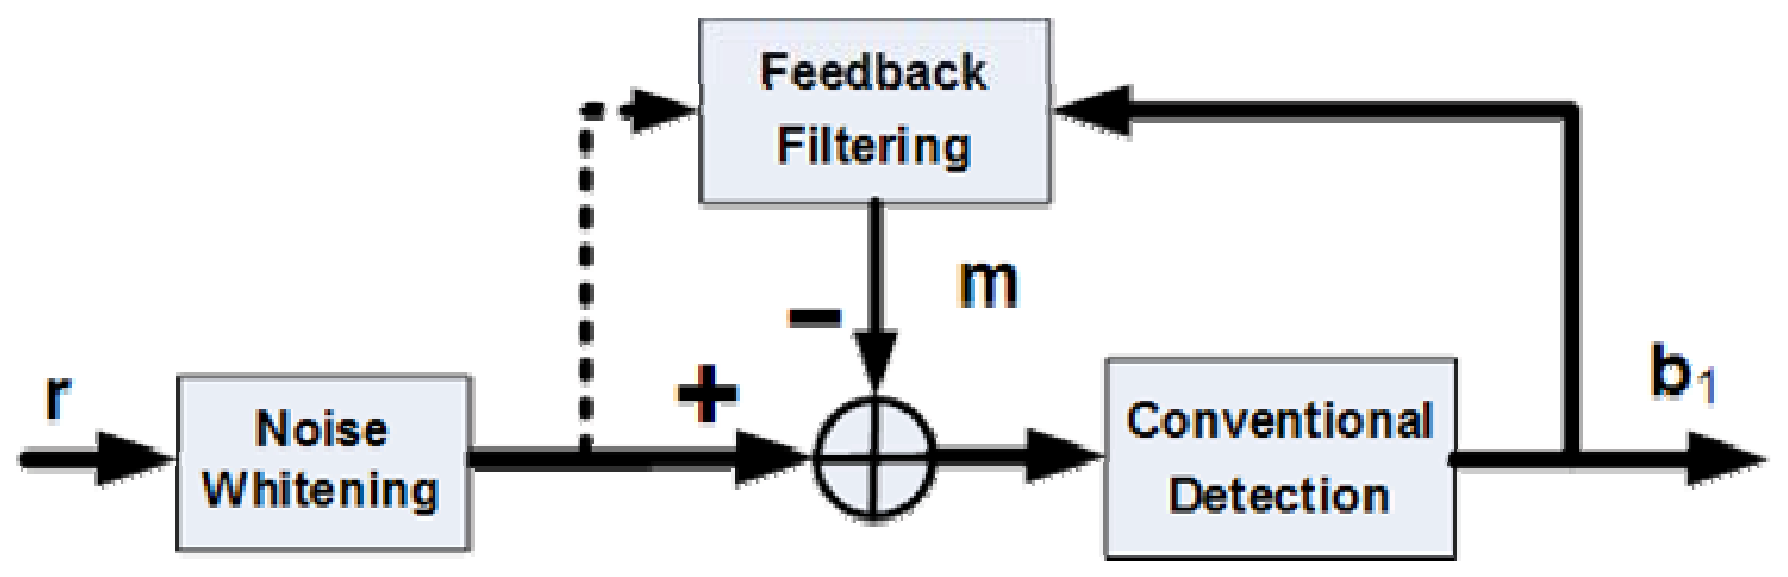
\includegraphics[width=3.2in]{BDFIC1.eps}
\caption{A decision feedback interference cancellation block
diagram} }\label{DFIC}
\end{figure}
\subsection{\em Least Squares Interference Cancellation}
In traditional least squares estimations, the observation matrix
is assumed to be error-free and all estimation errors are supposed
to come from $\br$. This can be formulated by
\begin{equation}\hspace{-0.09in}
\begin{array}{rcl}
\left[\matrix{{\bd}_{1\rm LS}\cr\bbf_{\rm
LS}}\right]&=&\mbox{arg}\min\limits_{\bx}\left\|\br-\bG\bx\right\|_2
\end{array}\label{prob_LS}
\end{equation}
\noindent where
\begin{equation}
\begin{array}{rcl}
\bG&=&\left[\matrix{\bS_1&\left(\bcS-\bS_1\bD_1\right)}\right]
\end{array}.
\end{equation}
\noindent Now $\bd_1$ as well as $\bbf$ can therefore be estimated
by
\begin{equation}\hspace{-0.0in}
\begin{array}{rcl}
\left[\matrix{{\bd}_{1\rm LS}\cr\bbf_{\rm
LS}}\right]&=&\bG^{+}\br.
\end{array}\label{b_LS_IC}
\end{equation}

Besides the traditional LS assumption, another one is to assume
both $\bG$ and $\br$ are noise-polluted so that (\ref{prob_LS})
becomes the total least squares (TLS) problem
\begin{equation}\hspace{-0.12in}
\begin{array}{rcl}
\left[\matrix{{\bG}_{\rm TLS}\cr\left[\matrix{{\bd}_{1\rm
TLS}\cr\bbf_{\rm
TLS}}\right]}\right]&=&\mbox{arg}\min\limits_{\bY,\
\bx}\left\|\left[\matrix{\bG\cr\br}\right]-\left[\matrix{\bY\cr\bY\bx}\right]\right\|_2
\end{array}.\label{prob_TLS}
\end{equation}
Let $\bG=\bU^{'}\mathbf{\Sigma}^{'}\bV^{'\rm T}$ and $[\bG\
\br]=\bU\mathbf{\Sigma}\bV^{\rm T}$ be the SVD of $\bG$ and $[\bG\
\br]$, respectively. If $\sigma_K^{'}
> \sigma_{K+1}$, the TLS estimation of $\bd_{1}$ and $\bbf$ is
\begin{equation}
\begin{array}{rcl}
\left[\matrix{{\bd}_{1\rm TLS}\cr\bbf_{\rm
TLS}}\right]&=&\left(\bG^{\rm
T}\bG-\sigma_{K+1}^2\bI\right)^{-1}\bG^{\rm T}\br
\end{array}
\end{equation}

It seems that either (\ref{prob_LS}) or (\ref{prob_TLS}) is not
accurate since $\bS_1$ is known to be noise-free and $\bcS$ is
noise-corrupted. It seems that it is more reasonable to require
$\bS_1$ to be unperturbed while keep $\bcS$ estimated. Therefore
it leads to a mixed least squares (MLS) interference cancellation
problem expressed by
\begin{equation}\hspace{-0.07in}
\begin{array}{l}
\left[\matrix{{\bcS}_{\rm
MLS}\cr\left[\matrix{{\bd}_{1}+\bD_{1}\bbf\cr\bbf}\right]_{\rm
MLS}}\right]=\mbox{arg}\min\limits_{\bZ,\
\by}\left\|\left[\matrix{\bcS\cr\br}\right]-\left[\matrix{\bZ\cr\left[\bS_1\
\bZ\right]\by}\right]\right\|_2
\end{array}.
\end{equation}
\noindent If $\sigma_{K-G}'>\sigma_{K-G+1}$, the MLS estimation of
$\bbf$ is
\begin{equation}\hspace{-0.070in}
\begin{array}{l}
{\bbf_{\rm MLS}}=\left(\bcS^{\rm H}\bQ_{12}\bQ_{12}^{\rm
H}\bcS-\sigma_{K-G+1}^{2}\bI\right)^{-1}\bcS^{\rm
H}\bQ_{12}\bQ_{12}^{\rm H}\br
\end{array}\label{f_MLS}
\end{equation}
\noindent where $\sigma_{K-G}'$ and $\sigma_{K-G+1}$ are the
$(K-G)$th and $(K-G+1)$th largest singular value of $\bQ_{12}^{\rm
H}\bcS$ and $\bQ_{12}^{\rm H}\left[\matrix{\br&\bcS}\right]$. The
MLS-IC ${\bd}_{1\rm MLS}$ can be expressed by
\begin{equation}\hspace{0.0in}
\begin{array}{rcl}
{\bd}_{1\rm
MLS}&=&\bS_{1}^{+}\br-\bS_{1}^{+}\left({\bcS}-{\bS}_{1}{\bD_1}\right){\bbf_{\rm
MLS}}
\end{array}\label{b_MLS_IC}
\end{equation}
\subsection{\em Maximum Likelihood Interference Cancellation}
In maximum likelihood interference cancellation (ML-IC), $\bd_1$
is estimated with maximizing the probability density function
(PDF) $p(\br;\ \bd_{1},\ \bbf)$. It is known that ML estimator
asymptotically is the minimum variance unbiased (MVU) estimator
though it is not optimal in general. For the linear Gaussian
signal model in (\ref{br_bm}), ML-IC can be written by
\begin{equation}\hspace{-0.12in}
\begin{array}{rcl}
\left[\matrix{{\bd}_{1\rm ML}\cr\bbf_{\rm
ML}}\right]&=&\mbox{arg}\min\limits_{\bx}\left\{\mathbf\delta^{\rm
H}\bR_{\bar\bn}\mathbf\delta\right\}
\end{array}
\end{equation}
\noindent where the estimation error vector
\begin{equation}
\begin{array}{rcl}
\mathbf\delta&=&\br-\bG\bx
\end{array}.
\end{equation}
Therefore the ML estimation of $\bd_1$ can be given by
\begin{equation}
\begin{array}{rcl}
\left[\matrix{{\bd}_{1\rm ML}\cr\bbf_{\rm
ML}}\right]&=&\left(\bG^{\rm
H}\bR_{\bar\bn}\bG\right)^{-1}\bG^{\rm H}\bR_{\bar\bn}^{-1}\br
\end{array}.\label{b_ML_IC}
\end{equation}

\subsection{\em Mini. Mean-Square Error Interference Cancellation}
With MMSE criterion, $\bd_{1}$ is estimated with minimizing the
Bayesian mean squared error (BMSE):
\begin{equation}\hspace{-0.0in}
\begin{array}{rcl}
\be_{\rm
BMSE}&=&\mbox{E}\left\|\left[\matrix{\hat\bd_{1}\cr\hat\bbf}\right]-\left[\matrix{\bd_{1}\cr\bbf}\right]\right\|_2^2
\end{array}.
\end{equation}
\noindent The MMSE estimation can then be written by
\begin{equation}\hspace{-0.15in}
\begin{array}{l}
\left[\matrix{{\bd}_{1\rm MMSE}\cr\bbf_{\rm
MMSE}}\right]=\mbox{arg}\min\limits_{\bx}\mbox{E}\left\|\br-\bG\bx\right\|_2
\end{array}\label{MMSE_IC}
\end{equation}
\noindent and, if $\br$, $\bd_{1}$ and $\bbf$ are jointly
Gaussian, it can be solved by
\begin{equation}
\begin{array}{rcl}
\left[\matrix{{\bd}_{1\rm MMSE}\cr\bbf_{\rm
MMSE}}\right]&=&\left(\bR_{\bx}+\bG^{\rm
H}\bR_{\bar\bn}\bG\right)^{-1}\bG^{\rm H}\bR_{\bar\bn}^{-1}\br
\end{array}\label{b_MMSE_IC}
\end{equation}
\noindent where
\begin{equation}
\begin{array}{rcl}
\bR_{\bx}&=&\mbox{E}\left\{\left[\matrix{\bd_{1}\bd_{1}^{\rm
H}&\bd_{1}\bbf^{\rm H} \cr \bbf\bd_{1}^{\rm H}&\bbf\bbf^{\rm
H}}\right]\right\}
\end{array}.%\label{b_ML_IC}
\end{equation}
\section{Implementation Issues}
\subsection{\em Adaptive Detection}
When transmitted signals experience channel condition changes, it
is better for the receiver to response fast enough to follow this
change with minimum adaptive lag. With (\ref{bcs}) and
(\ref{br_bm}), it shows that the proposed DFIC framework $M$
previously received symbols for the next detection so that it may
be able to track channel fast. Since its implementations typically
involve the inverse of $\bG^{\rm H}\bG$ in (\ref{b_LS_IC}),
$\bG^{\rm H}\bR_{\bar\bn}\bG$ in (\ref{b_ML_IC}), etc., one of the
possible approaches is to follow the well-known
Sherman-Morrison-Woodbury matrix inverse
lemma~\cite{Haykin96,Wang05B}. For example, if we define
\begin{equation}
\begin{array}{rcl}
\bPhi[n]&=&\bG^{\rm H}[n]\bG[n]
\end{array},\label{R_G}
\end{equation}
\noindent where $\bG[n]$ denotes the instance of $\bG$ at $t=n$,
so that $\bPhi[n+1]$ can be rewritten by
\begin{equation}
\begin{array}{rcl}
\bPhi[n+1]&=&\bPhi[n] + \bu[n]\bu^{\rm H}[n]
\end{array}.
\end{equation}
The inverse of $\bPhi[n+1]$ can be recursively calculated by
\begin{equation}\hspace{-0.08in}
\begin{array}{l}
\bPhi^{-1}[n+1]=\bPhi^{-1}[n]-\frac{\bPhi^{-1}[n]\bu[n]\bu^{\rm
H}[n]\bPhi^{-1}[n]}{1+\bu^{\rm H}[n]\bPhi^{-1}[n]\bu[n]}
\end{array}.\label{adaptiveLS}
\end{equation}
\subsection{\em Iterative Detection}
The presented detection framework can be generalized by solving
the following optimization problem:
\begin{equation}
\begin{array}{rcl}
\hat{\bd}_{1}&=&\min{f\left(\br;\ \bcS,\hat{\bD}_1\right)}
\end{array},\label{generalFramework}
\end{equation}
\noindent which subject to some possible constraints, where the
$f\left(\cdot\right)$ is the objective function. Iterative
detection is one the approaches for solving this optimization
problem. For this, (\ref{generalFramework}) may be extended to
\begin{equation}
\begin{array}{rcl}
\hat{\bd}_{1}&=&\min{f\left(\br;\ \left[\bcS\
\br\right],\left[\hat{\bD}_1\ \hat{\bd}_1\right]\right)}
\end{array}.\label{extendedFramework}
\end{equation}
And one iterative framework for solving (\ref{extendedFramework})
can be expressed by
\begin{equation}\hspace{-0.05in}
\begin{array}{rcl}
\hat{\bd}_{1}[n+1]&=&\min{f\left(\br;\ \left[\bcS\
\br\right],\left[\hat{\bD}_1\ \hat{\bd}_1[n]\right]\right)}
\end{array}.
\end{equation}
\subsection{\em Coded Blind Interference Cancellation}
Actually, an IC detector will cancel the interfering signal
exactly provided that the decision was correct and channel
information is known. Otherwise, it may increase the contribution
of the interferers. This means that the previous detection results
of $\bD_{1}$ are critical here. Therefore, some coding/decoding
schemes may be applied with detecting $\bD_{1}$ before the next
detection.
\section{Performance Analysis}
\subsection{\em Comparison with Existing Blind Detectors}
\begin{figure*}[t]\label{SchemComp}\small
\center{Table 1. The comparison of the proposed framework and
other detection approaches}
\begin{center}
\begin{tabular}{lcccc}
Parameters & Conv. DF-IC & Blind MMSE & Subspace Approaches & Blind DF-IC\\
\hline \hline
Signature of desired user(s) & $\bf\Box$ & $\mathbf\Box$ &  $\mathbf\Box$ & $\mathbf\Box$ \\
Signature of other users & $\mathbf\Box$ & &  \\
Timing of desired user(s)  & $\mathbf\Box$ & $\mathbf\Box$ & $\mathbf\Box$ & $\mathbf\Box$ \\
Timing of other users  & $\mathbf\Box$ & & & \\
Received amplitudes  & $\mathbf\Box$ & &  &\\
ECC decoding-integratable& $\mathbf\Box$ &&& $\mathbf\Box$ \\
Initialization~{\small *} &  & $\ge L$ & $\ge L$ & $M$\\
Latency & $K$ & $1$ & $1$ & $1$ \\
Complexity order & $K$ & $1$ & $1$ & $1$ \\
\hline \hline \multicolumn{5}{l}{\tiny * For blind MMSE or
subspace approaches, they typically require much more than $L$
signals before their first detection.}
\end{tabular}
\end{center}
\end{figure*}
The comparison between the proposed framework and other major
schemes is presented in Table~1. The proposed framework only
requires $M$, where $L\ge M\ge (K-G)$, previous received signal
for signal detection and its complexity is closed to conventional
detectors while other blind approaches typically requires a lots
more than $L$ signals~\cite{Madh94,Wang98,Zhang02}.
\subsection{\em Noise Enhancement}
It is known that there is a noise enhancement issue in LS-based
decorrelating detection. With conventional decorrelating
detection, the output signal-to-noise ratio (SNR) for user $k$ is
decreased by $\left[\bR_{\bs}^{+}\right]_{kk}$. Due to the noise
item $\bN$ in $\bcS$, there is an additional noise enhancement in
the proposed LS-DFIC.

Following Girko's Law, providing $\alpha=\frac{K-G}{M}$ is fixed,
the diagonal element of
$\frac{1}{M}\left(\bB_2^{+}\bb_2\right)\left(\bB_2^{+}\bb_2\right)^{\rm
H}$ can be approximated to be $1-\alpha$ with $K$, $M$
$\rightarrow\infty$~\cite{Muller}. Therefore the covariance matrix
of $\bar\bn$ can be expressed by
\begin{equation}
\begin{array}{rcl}
\bR_{\bar\bn}&=&\frac{2M+K-G}{M}\sigma^{2}\bI
\end{array}.\label{noise_var_new}
\end{equation}
\noindent Since $\frac{2M+K-G}{M}\sigma^{2}>\sigma^{2}$, the
receiver output noise is enhanced.
\subsection{\em AME and Near-Far Resistance}
A commonly used performance measure for a multiuser detector is
asymptotic multiuser efficiency (AME) and NFR~\cite{Verd98}. The
AME of the proposed schemes is
\begin{equation}
\begin{array}{rcl}
\bar{\eta}_k&=&{\frac{M}{2M+G-K}}\left[\bR_{\bs}^{+}\right]_{kk}^{-1}
\end{array}.
\end{equation}
\subsection{\em CRLB for $\bd_1$ and $\bbf$ Estimation}
The Cram\'{e}r-Rao Lower Bound (CRLB) is given by the inverse of
the Fisher information matrix (FIM). Providing $\bcS$ and $\bD_1$
are known beforehand, we first define the parameter vector
$\mathbf{\phi} = \left[\bar{\sigma}^{2}\ \bd_1^{\rm T}\ \bbf^{\rm
T}\right]^{\rm T}$, where $\bar{\sigma}^{2}
=(1+\frac{M}{M+G-K})\sigma^{2}$, for computing the FIM
\begin{equation}
\begin{array}{rcl}
{\bI(\mathbf{\phi})} &=& {\rm E} \left\{ \left( \frac{\partial
\ln{\cal L}}{\partial \mathbf{\phi}} \right) \left( \frac{\partial
\ln{\cal L}}{\partial \mathbf{\phi}} \right)^{\rm T} \right\}
\label{fim}
\end{array}
\end{equation}
\noindent where $\ln{\cal L}$ is the log-likelihood function given
by
\begin{equation}
\begin{array}{rcl}
\ln{\cal
L}&=&C-L\ln\bar{\sigma}^2-\frac{1}{2\bar{\sigma}^2}\parallel\mathbf{e}\parallel_2^2
\end{array},\label{logl}
\end{equation}
\noindent $C$ is a constant and
$\mathbf{e}=\br-\bS_1\bd_1+(\bcS-\bS_1\bD_1)\bbf$. Providing
$\bcS$ and $\bD_1$ are known, the closed-form CRLB expression of
$\bd_1$ is then given by
\begin{equation}
\begin{array}{l}
{\rm CRLB}\left(\bx\ \big\arrowvert\ \bcS,\
\bD_1\right)=(1+\frac{M}{M+G-K})\sigma^{2}\left(\bG^{\rm
H}\bG\right)^{\rm +}
\end{array}.\label{CRLB_f}
\end{equation}
\noindent where $\bx=\left[\matrix{\bd_1^{\rm T}&\bbf^{\rm
T}}\right]^{\rm T}$.
\section{Computer Simulations}
There are $K=10$ users with the group size $G=3$ and the spreading
sequences used in simulations are $64$-chip ($L=64$) random
sequences. In the computer simulations, the previous $M$ amplitude
estimates are averaged for the next detection without additional
amplitude filtering. From Fig. 2, it shows that the performance of
the MMSE interference cancellor is comparable to single-user
matched filter (SU-MF) and the decorrelating detector when
interfering signal power is small. When the interfering signal
power becomes larger, the SU-MF suffers from the near-far issue
and BER performance become very bad since its near-far resistance
is small. However, the MMSE interference cancellor as well as the
LS interference cancellor still works very well with strong
near-far resistance. In Fig. 3, the near-far resistance of the
proposed interference cancellors is checked with changing
interfering signal power. We can see that the both the LS-based
and MMSE-based interference cancellors have good resistance to
interferences. But compared with the conventional decorrelating
detection, these decision-feedback interference cancellors have a
higher noise floor. This is also confirmed in the previous
analysis.
\begin{figure}\hspace{-0.5in} \center{
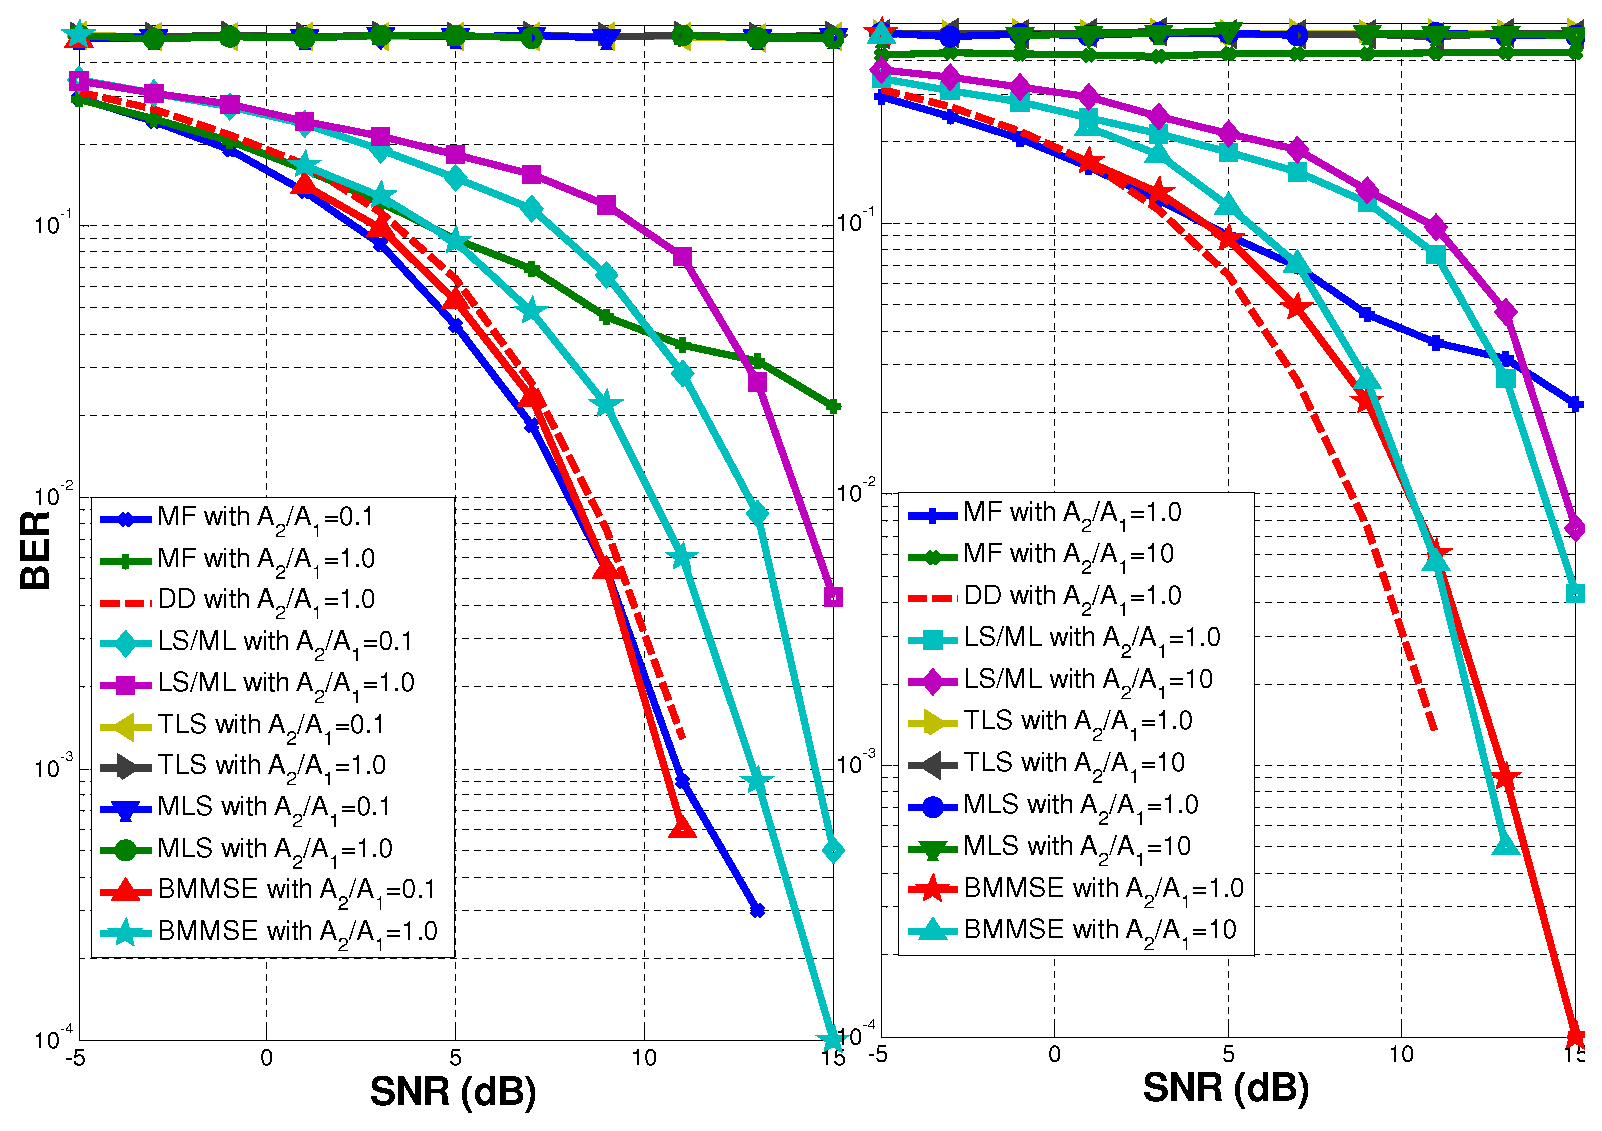
\includegraphics[width=3.25in]{BER_40_10_3_D.eps}
\caption{ The performance of the proposed blind DF-ICs against
SNR, $G=3$, $K=10$ and $M=40$. } }\label{BER_SNR}
\end{figure}
\begin{figure} \center{
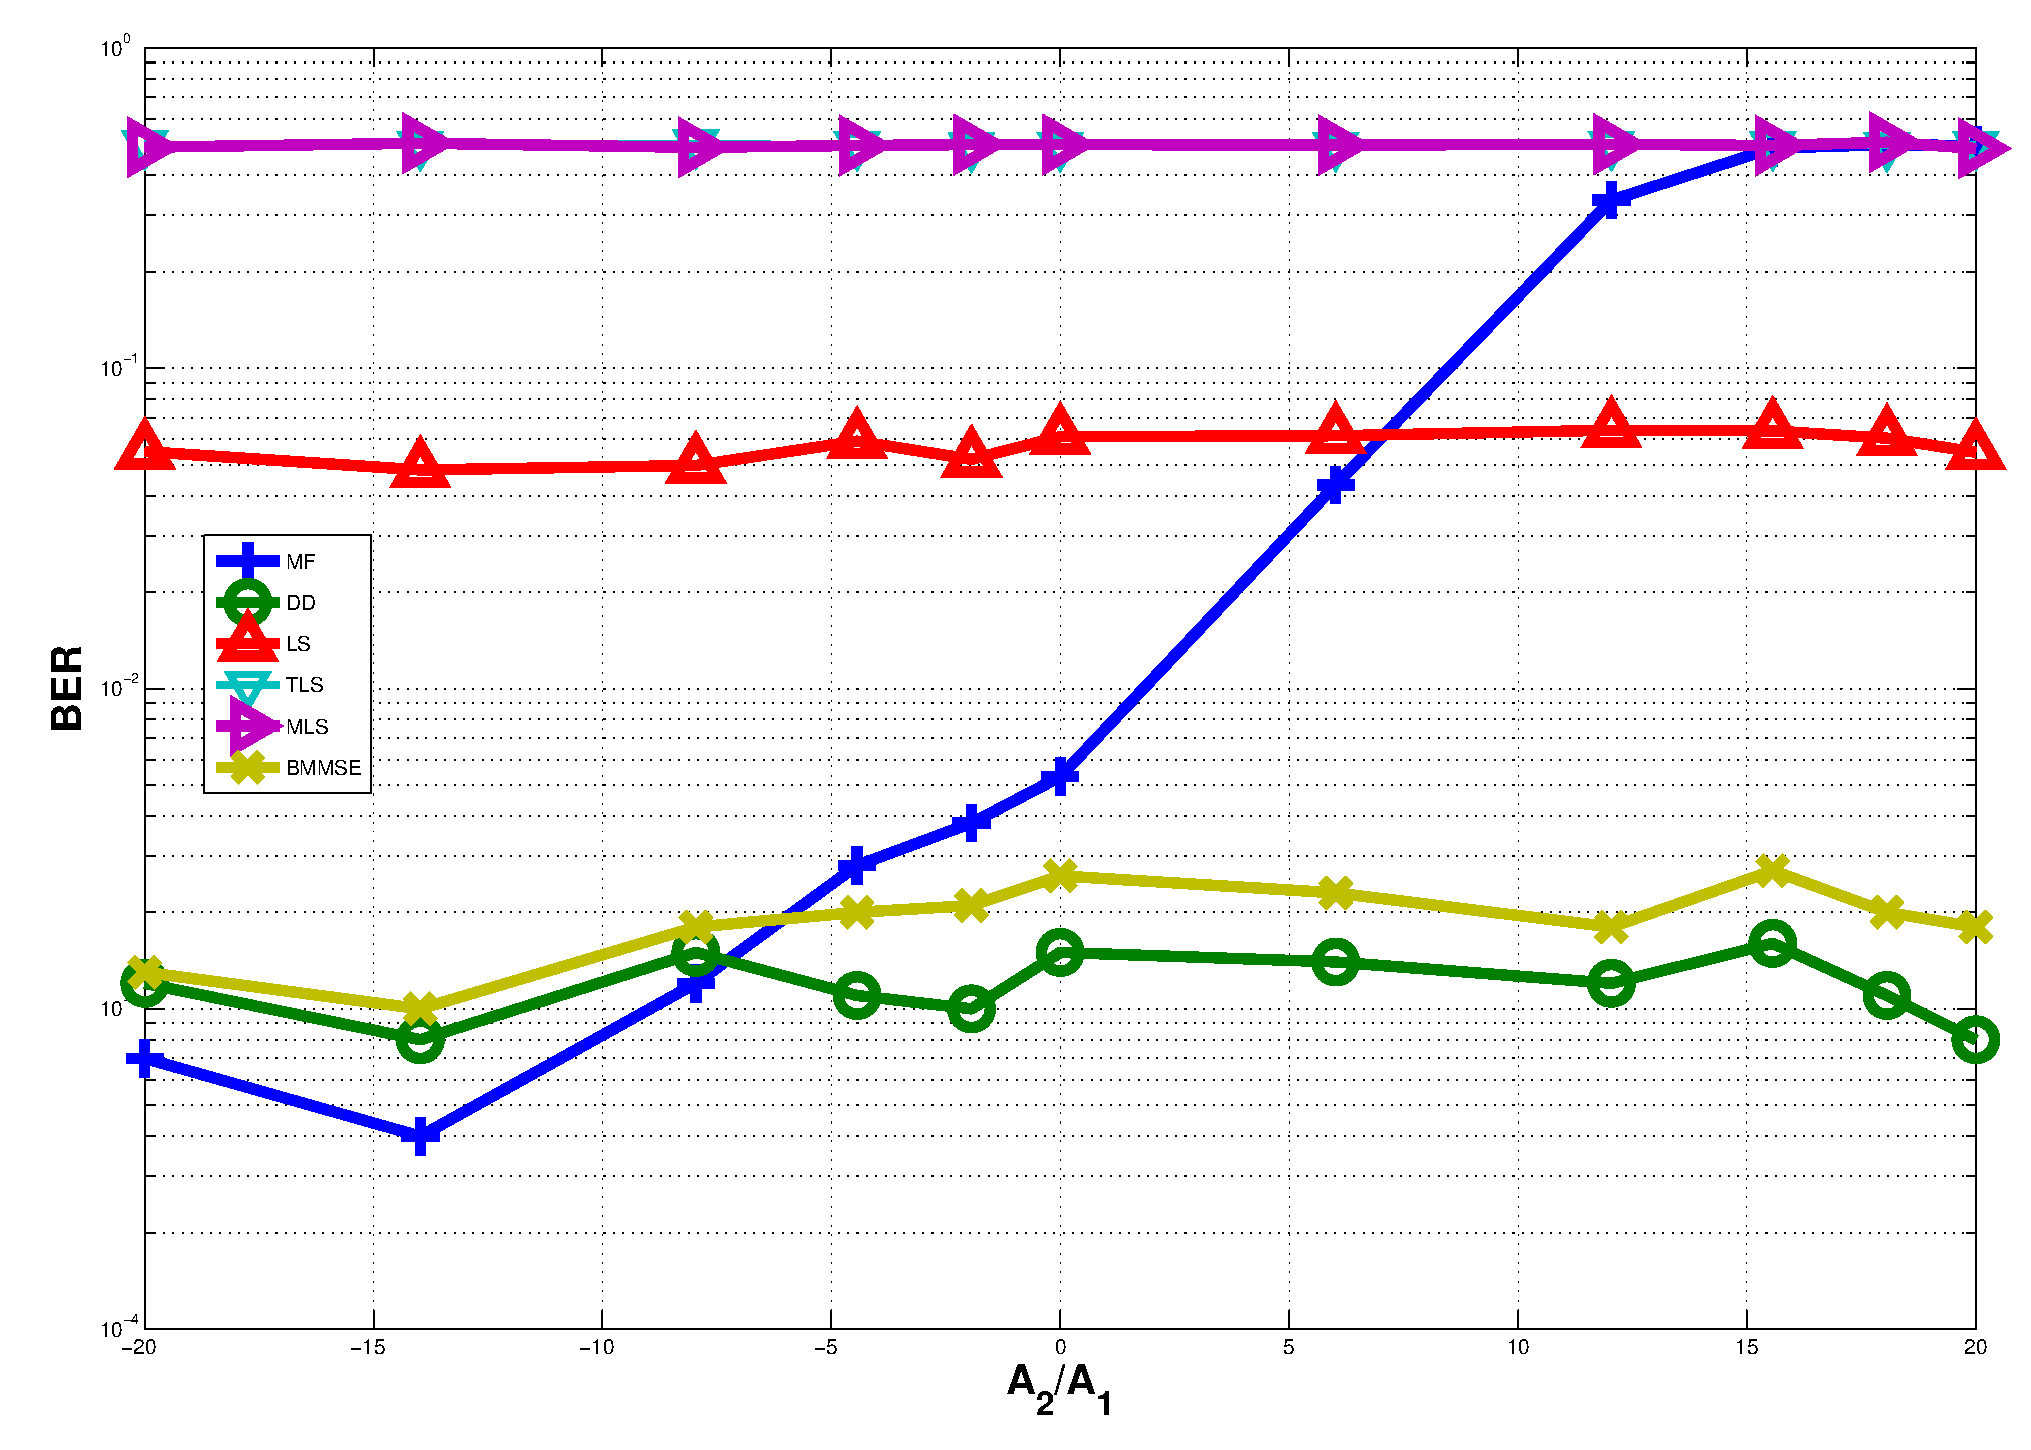
\includegraphics[width=2.5in]{NFR_10_40_2_1.eps}
\caption{ The near-far resistance performance of the proposed
DF-IC, $M=40$, $K=2$, $G=1$ and ${\rm SNR}=10{\rm dB}$.}
}\label{BER_A_SNR}
\end{figure}
\section{Conclusions}
In this paper, we proposed a blind interference cancellation
framework as well as several implementations. They are simple and
direct and require a minimum amount of previous detected symbols.
The implementation considerations, the performance analysis and
computer simulations of the proposed schemes are also presented.
\small\bibliographystyle{unsrt}
\bibliography{FastBDD,InterferenceCancellation}
\end{document}
